\documentclass[a4paper,landscape]{article}
\usepackage[margin=0.8cm]{geometry}
\usepackage{tikz}
\usepackage{tikzfill}

\newcommand\wallHeight{5.62cm}
\newcommand\coverHeight{2.00cm}
\newcommand\buildingHeight{7.62cm} % must be wallHeight + coverHeight, and I want it to be 3in = 7.62cm
\newcommand\buildingWidth{17.9cm}
\newcommand\buildingDepth{10cm}

\newcommand\innerEps{0.5mm}
\newcommand\norm{1}
\newcommand\flip{-1}
\newcommand\flapWidth{0.8cm}
\newcommand\vflap[4]
{
\draw (#1, #2)
  -- ++(#4 * \flapWidth, -\flapWidth)
  -- ++(0, -#3 + 2 * \flapWidth)
  -- ++(#4 * -\flapWidth, -\flapWidth)
  -- cycle
  ;
}

\begin{document}
\pagestyle{empty}
\begin{tikzpicture}
  [ remember picture
  , overlay
  , line width=0.02cm
  ]

%%%%% Walls

\begin{scope}
\vflap{0}{0}{\buildingHeight}{\flip}
%\path[draw,fill tile image*={width=\buildingDepth}{/home/mkl/sandbox/tabletop/terrain/textures/concrete/PaintedPlaster010_1K-JPG_Color.jpg}] (0,0)
\draw (0,0)
  rectangle ++(\buildingWidth,-\buildingHeight)
  rectangle ++(\buildingDepth,\buildingHeight)
  ;
\end{scope}

\begin{scope}[yshift=-9cm]
\vflap{0}{0}{\buildingHeight}{\flip}
%\path[draw,fill tile image*={width=\buildingDepth}{/home/mkl/sandbox/tabletop/terrain/textures/concrete/PaintedPlaster010_1K-JPG_Color.jpg}] (0,0)
\draw (0,0)
  rectangle ++(\buildingWidth,-\buildingHeight)
  rectangle ++(\buildingDepth,\buildingHeight)
  ;
\end{scope}

\end{tikzpicture}


\newpage


\begin{tikzpicture}
  [ remember picture
  , overlay
  , line width=0.02cm
  ]


%%%%% Stabilizing Cross

\begin{scope}[yshift=0.5cm]
\draw (0, 0)
  rectangle ++(\buildingWidth - \innerEps,-\wallHeight)
  ;
\draw (\buildingWidth/2 + \innerEps/2, 0) -- ++(0, -\wallHeight/2);
\vflap{0}{0}{\wallHeight}{\flip}
\vflap{\buildingWidth - \innerEps}{0}{\wallHeight}{\norm}
\end{scope}

\begin{scope}[yshift=-0.5cm, xshift=27.5cm, rotate=-90]
\draw (0, 0)
  rectangle ++(\buildingDepth - \innerEps,-\wallHeight)
  ;
\draw (\buildingDepth/2 + \innerEps/2, 0) -- ++(0, -\wallHeight/2);
\vflap{0}{0}{\wallHeight}{\flip}
\vflap{\buildingDepth - \innerEps}{0}{\wallHeight}{\norm}
\end{scope}


%%%%% Roof

\begin{scope}[yshift=-\buildingHeight + 2.0cm,xshift=-0.5cm]
%\path[draw,fill tile image*={height=8cm}{/home/mkl/sandbox/tabletop/terrain/textures/solar-panel/SolarPanel003_1K-JPG_Color.jpg}] (\coverHeight,0)
\draw (\coverHeight,0)
  rectangle ++(\buildingWidth - \innerEps,-\coverHeight)
  rectangle ++(-\buildingWidth + \innerEps,-\buildingDepth + \innerEps)
  rectangle ++(\buildingWidth - \innerEps,-\coverHeight)
  ;
%\path[draw,fill tile image*={height=8cm}{/home/mkl/sandbox/tabletop/terrain/textures/solar-panel/SolarPanel003_1K-JPG_Color.jpg}] (0, -\coverHeight)
\draw (0, -\coverHeight)
  rectangle ++(\coverHeight,-\buildingDepth + \innerEps)
  ;
%\path[draw,fill tile image*={height=8cm}{/home/mkl/sandbox/tabletop/terrain/textures/solar-panel/SolarPanel003_1K-JPG_Color.jpg}] (\buildingWidth + \coverHeight - \innerEps, -\coverHeight)
\draw (\buildingWidth + \coverHeight - \innerEps, -\coverHeight)
  rectangle ++(\coverHeight,-\buildingDepth + \innerEps)
  ;
\end{scope}

\end{tikzpicture}

\end{document}
